\chapter{The Braid Group}\label{ch:braid_group}

\begin{definition}
    The \textit{configuration space} of $n$ ordered distinct points in the complex plane $\C$ is defined as $M_n = \left\{ \left( z_1,\dots,z_n \right)\in\C ; z_i\neq z_j,\forall i\neq j \right\}$. Alternatively, consider $\mathcal{D}$ to be the collection of all hyperplanes $H_{i,j}=\left\{ z_i=z_j \right\}\in\C^n$ for $1\leq i < j \leq n$. Then we can define $M_n = \C^n \setminus \mathcal{D}$.
\end{definition}

Note that $\left( z_1,z_2,z_3,\dots,z_n \right)$ and $\left( z_2,z_1,z_3,\dots,z_n \right)$ are different points in the configuration space $M_n$. Before studying the various interpretations of the braid group, we first define the braid group itself.

\begin{definition}
    The \textit{pure braid group} on $n$ strands, denoted $PB_n$, is the fundamental group of $M_n$. One can write $PB_n = \pi_1(M_n)$.
\end{definition}

\section{Visualization of pure braids}

We can think of a pure braid as a loop in $M_n$:
\begin{align*}
    \beta : \left[ 0,1 \right] &\to M_n \\
    t &\mapsto \beta(t) = \left( \beta_1(t),\beta_2(t),\dots,\beta_n(t) \right),
\end{align*}
with some base point. Conventionally, we define the base point as the $n$-tuple of integers $(1,2,3,\dots,n)\in \C^n$. Then a pure braid can be though of the motion of these points in the complex plane as $t$ ranges from 0 to 1 in which $\beta_i(t)$ is defined and $\beta_i(t)\neq \beta_j(t)$ for every $t\in[0,1]$ and $i\neq j\in\left\{ 1,2,\dots,n \right\}$. Because each $\beta_i$ is a loop, it must start and end at the point $i$ (e.g., $\beta_i(0)=\beta_i(1)=i$). Recall that the loops are actually equivalence classes of loops under homotopy. As a result, we can continuously deform the motion of the $n$ points while maintaining the same pure braid (up to equivalence) so long as we preserve the pairwise distinction of the points for all time $t\in[0,1]$.

A common visualization of pure braids is to plot the motion of the points in 3-dimensional space. For each $t\in [0,1]$, we draw the points $\left( \beta_i(t),t \right)$ in $\C\times[0,1]$ for every $i\in\left\{ 1,\dots,n \right\}$. The space $\C\times[0,1]$ can be thought of as a spacetime diagram, where the motion of the points is plotted in the complex plane at each time $t$, with the time being the vertical axis. The convention is to have $\C\times\left\{ 0 \right\}$ placed above $\C\times\left\{ 1 \right\}$, so that the motion of the points is plotted from top to bottom, as in \cref{fig:C_pure_braid}.

\begin{figure}[htbp]
    \centering
    \usetikzlibrary{shapes.geometric}
\begin{tikzpicture}[
    braid/.cd,
    crossing convention=under,
    crossing height = .75cm,
    gap = .075,
    ultra thick
]
\pic (b) {braid={s_1 s_2^{-1} s_1 s_2^{-1} s_1 s_2^{-1}}};

\foreach \i in {1,...,3} {
    \fill (b-\i-s) circle (2pt) node[above] {$\i$};
    \fill (b-\i-e) circle (2pt);
}

\coordinate (t1) at ($(b-1-s) + (-.25cm,.5cm)$);
\coordinate (t2) at ($(b-3-s) + (1cm,.5cm)$);
\coordinate (t3) at ($(b-3-s) + (.25cm,-.35cm)$);
\coordinate (t4) at ($(b-1-s) + (-1cm,-.35cm)$);

\coordinate (b1) at ($(b-1-e) + (-.25cm,.5cm)$);
\coordinate (b2) at ($(b-3-e) + (1cm,.5cm)$);
\coordinate (b3) at ($(b-3-e) + (.25cm,-.35cm)$);
\coordinate (b4) at ($(b-1-e) + (-1cm,-.35cm)$);

\draw[thick] (t1) -- (t2) -- (t3) -- (t4) -- cycle;
\draw[thick] (b1) -- (b2) -- (b3) -- (b4) -- cycle;

\node[left] at ($(t1)!.5!(t4)$) {$\C\times\left\{ 0 \right\}$};
\node[left] at ($(b1)!.5!(b4)$) {$\C\times\left\{ 1 \right\}$};

\end{tikzpicture}
    \caption{A pure braid on three strands is visualized as the trajectory of three particles as they move in $\C$, plotted over an arbitrary (normalized) time period. Each point ends at the same relative starting position in $\C$.}\label{fig:C_pure_braid}
\end{figure}

For every $i\in\left\{ 1,\dots,n \right\}$, the motion of a single point starting at $(i,0)$ and ending at $(i,1)$ is known as the $i$-th \textit{strand} of the pure braid. This can also be described by the $i$-th projection of the $n$-tuple $\beta(t)$. Thus, two braids are equivalent under homotopy if, for every moment of a continuous deformation of the $n$ strands in $\C\times [0,1]$, the (fixed) endpoints $((1,0),(2,0),\dots,(n,0))$ and $((1,1),(2,1),\dots,(n,1))$ are connected by strands that are pairwise disjoint where each strand intersects the plane $\C\times\left\{ t \right\}$ exactly once for every $t\in[0,1]$.

As pure braids are members of the pure braid group, multiplication is a well-defined operation. In the context of $M_n$, multiplication of pure braids involves the concatenation of loops. Visually, this is the process of stacking braids on top of each other, and then rescaling the time dimension so that $t$ ranges from 0 to 1.

\section{General braids}
In the previous section, we defined pure braids in which the endpoints of each strand are identical at the beginning and end of the motion. This notion generalizes to define (non-pure) braids. First, we define a more general configuration space than $M_n$. The symmetric group $S_n$ permutes the $n$ distinct points in $\C$. Then the \textit{configuration space of n unordered points in $\C$} is the quotient space $N_n = M_n/S_n$.

\begin{definition}
    The braid group on $n$ strands is the fundamental group of $N_n$, denoted $B_n = \pi_1(N_n)$.
\end{definition}

The visualization of a braid is the same as in the case of pure braids, only now the endpoints of each strand do not necessarily match the starting points, as illustrated \cref{fig:C_general_braid}. For example, the $i$-th strand may start at the point $(i,0)$ but end at the point $(j,1)$ for $i,j\in\left\{ 1,\dots,n \right\}$. The equivalence of strands is still defined as before under the homotopy of loops. Loop concatenation defines the multiplication of braids, as before.

% \missingfigure[figwidth=6cm]{Gonzalez Figure 1}
\begin{figure}[htbp]
    \centering
    \usetikzlibrary{shapes.geometric}
\begin{tikzpicture}[
    braid/.cd,
    crossing convention=under,
    crossing height = .825cm,
    gap = .0625,
    ultra thick
]
\pic (b) {braid={s_{1-3} s_4 s_3^{-1} s_2 s_1 s_2^{-1} s_4}};

\foreach \i in {1,...,5} {
    \fill (b-\i-s) circle (2pt) node[above] {$\i$};
    \fill (b-\i-e) circle (2pt);
}

\coordinate (t1) at ($(b-1-s) + (-.25cm,.5cm)$);
\coordinate (t2) at ($(b-5-s) + (1cm,.5cm)$);
\coordinate (t3) at ($(b-5-s) + (.25cm,-.35cm)$);
\coordinate (t4) at ($(b-1-s) + (-1cm,-.35cm)$);

\coordinate (b1) at ($(b-5-e) + (-.25cm,.5cm)$);
\coordinate (b2) at ($(b-2-e) + (1cm,.5cm)$);
\coordinate (b3) at ($(b-2-e) + (.25cm,-.35cm)$);
\coordinate (b4) at ($(b-5-e) + (-1cm,-.35cm)$);

\draw[thick] (t1) -- (t2) -- (t3) -- (t4) -- cycle;
\draw[thick] (b1) -- (b2) -- (b3) -- (b4) -- cycle;

\node[left] at ($(t1)!.5!(t4)$) {$\C\times\left\{ 0 \right\}$};
\node[left] at ($(b1)!.5!(b4)$) {$\C\times\left\{ 1 \right\}$};

\end{tikzpicture}
    \caption{A general braid on five strands. The ending position of each particle is not necessarily in the same location of $\C$ as the starting position, which classifies this as a general braid.}\label{fig:C_general_braid}
\end{figure}

Note that for $n\geq 1$ there is a natural inclusion $\iota:B_n\hookrightarrow B_{n+1}$ in which we add a new strand to any $\beta\in B_n$ that does not interact with the other strands.

\section{Standard generators of the braid group}\label{sec:std_gens}
Originally proposed by Artin~\cite{Artin1947}, each braid can be decomposed into a product of \textit{standard generators} of the braid group. When visualizing braids in $\R\times[0,1]$, a crossing of two strands is clearly indicated by one going over the other, as in \cref{fig:Gen_on_Strands}. Suppose each crossing occurs at a different time $t\in[0,1]$. Then by rescaling the time component of an arbitrary braid, we can decompose it into a stack of simple braids with only one crossing between neighboring strands per braid. Each single crossing of strands can be obtained by performing a transposition between neighboring endpoints of the strands.

% \missingfigure[figwidth=6cm]{Gonzalez Figure 2}
\begin{figure}[htbp]
    \centering
    \def\sep{.5cm}
\def\corners{4*\sep}
\def\hscale{.5}
\def\g{.05cm}

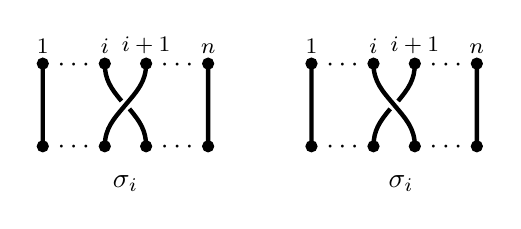
\begin{tikzpicture}
    \begin{scope}[shift={(-\corners-2.5*\sep,0)}]
        \coordinate (center) at (0,0);
        \coordinate (1s) at (-\corners, \hscale*\corners);
        \coordinate (ns) at (\corners, \hscale*\corners);
        \coordinate (1e) at (-\corners, -\hscale*\corners);
        \coordinate (ne) at (\corners, -\hscale*\corners);
        \coordinate (is) at (-\sep, \hscale*\corners);
        \coordinate (ip1s) at (\sep, \hscale*\corners);
        \coordinate (ie) at (-\sep, -\hscale*\corners);
        \coordinate (ip1e) at (\sep, -\hscale*\corners);
        \coordinate (gap) at (\g,-\g);

        \filldraw
            (1s) circle (2pt) node[above, font=\footnotesize] {$1$}
            (ns) circle (2pt) node[above, font=\footnotesize] {$n$}
            (1e) circle (2pt)
            (ne) circle (2pt)
            (is) circle (2pt) node[above, font=\footnotesize] {$i$}
            (ip1s) circle (2pt) node[above, font=\footnotesize] {$i+1$}
            (ie) circle (2pt)
            (ip1e) circle (2pt)
            (is) circle (2pt)
            (ip1s) circle (2pt)
            % ($(center) + (gap)$) circle (.6pt)
            % ($(center) - (gap)$) circle (.6pt)
            ;
            
        \node at ($(1s)!0.5!(is) - (0,.4725pt)$) {$\cdots$};
        \node at ($(ip1s)!0.5!(ns) - (0,.4725pt)$) {$\cdots$};
        \node at ($(1e)!0.5!(ie) - (0,.47pt)$) {$\cdots$};
        \node at ($(ip1e)!0.5!(ne) - (0,.47pt)$) {$\cdots$};
        \node[below, yshift=-5*\g] at ($(ie)!.5!(ip1e)$) {$\sigma_i$};
        
        \draw[ultra thick]
            (1s) -- (1e)
            (ns) -- (ne)
            [out=-90, in=130] (is) to ($(center) - (gap)$)
            [out=-50, in=90] ($(center) + (gap)$) to (ip1e)
            [out=-90, in=50] (ip1s) to (center)
            [out=-130, in=90] (center) to (ie);
    \end{scope}
    
    \begin{scope}[shift={(\corners+2.5*\sep,0)}]
        \coordinate (center) at (0,0);
        \coordinate (1s) at (-\corners, \hscale*\corners);
        \coordinate (ns) at (\corners, \hscale*\corners);
        \coordinate (1e) at (-\corners, -\hscale*\corners);
        \coordinate (ne) at (\corners, -\hscale*\corners);
        \coordinate (is) at (-\sep, \hscale*\corners);
        \coordinate (ip1s) at (\sep, \hscale*\corners);
        \coordinate (ie) at (-\sep, -\hscale*\corners);
        \coordinate (ip1e) at (\sep, -\hscale*\corners);
        \coordinate (gap) at (\g,\g);

        \filldraw
            (1s) circle (2pt) node[above, font=\footnotesize] {$1$}
            (ns) circle (2pt) node[above, font=\footnotesize] {$n$}
            (1e) circle (2pt)
            (ne) circle (2pt)
            (is) circle (2pt) node[above, font=\footnotesize] {$i$}
            (ip1s) circle (2pt) node[above, font=\footnotesize] {$i+1$}
            (ie) circle (2pt)
            (ip1e) circle (2pt)
            (is) circle (2pt)
            (ip1s) circle (2pt)
            % ($(center) + (gap)$) circle (.6pt)
            % ($(center) - (gap)$) circle (.6pt)
            ;
            
        \node at ($(1s)!0.5!(is) - (0,.4725pt)$) {$\cdots$};
        \node at ($(ip1s)!0.5!(ns) - (0,.4725pt)$) {$\cdots$};
        \node at ($(1e)!0.5!(ie) - (0,.47pt)$) {$\cdots$};
        \node at ($(ip1e)!0.5!(ne) - (0,.47pt)$) {$\cdots$};
        \node[below, yshift=-5*\g, xshift=1.75*\g] at ($(ie)!.5!(ip1e)$) {$\iv{\sigma_i}$};
        
        \draw[ultra thick]
            (1s) -- (1e)
            (ns) -- (ne)
            [out=-90, in=50] (ip1s) to ($(center) + (gap)$)
            [out=-130, in=90] ($(center) - (gap)$) to (ie)
            [out=-90, in=130] (is) to (center)
            [out=-50, in=90] (center) to (ip1e);
    \end{scope}
\end{tikzpicture}
    \caption{The action of $\sigma_i$ on $n$ strands. The $i$-th strand gets twisted behind the $(i+1)$-th strand when acted on by $\sigma_i$, and the opposite occurs for $\iv{\sigma_i}$. In that way, concatenating these two braids would result in no intertwining of strands, giving the identity braid.}\label{fig:Gen_on_Strands}
\end{figure}

For instance, swapping the endpoints of the $i$-th and $(i+1)$-th strands can be written as applying $\sigma_i$ to the identity braid (i.e., the braid that starts without any crossings of strands). It must be noted that there are two distinct ways to swap the endpoints of two strands. From a top-down perspective looking at the plane $\C\times\left\{ t \right\}$ for some time $t$, $\sigma_i$ swaps $(i,t)$ and $(i+1,t)$ in a clockwise rotation. The reverse of this operation (i.e., twisting the endpoints around in the counterclockwise direction) is denoted $\sigma_i^{-1}$. Both of these operations are illustrated in \cref{fig:Gen_on_Strands}. The standard generators of the braid group $B_n$ are defined as the set $\left\{ \sigma_1,\sigma_2,\dots,\sigma_{n-1} \right\}$. An arbitrary braid can be constructed by concatenating (or stacking) the simple braids made from the standard generators before rescaling the time coordinate to $[0,1]$.

\section{Automorphisms of the free group}\label{sec:Aut_Fn}

Consider the $n$-times punctured disk $\D_n$. The fundamental group of $\D_n$ involves loops that start and end at the same (fixed) base point in $\partial\D_n$. Up to homotopy, a clockwise-directional loop that encompasses the $i$-th hole in $\D_n$ corresponds to the $i$-th generator of the free group $F_n$ of rank $n$, which is illustrated in \cref{fig:Gen_on_Dn}. In fact, $\pi_1\left( \D_n \right) = F_n$. This equality allows us to define a representation of the braid group on $n$ strands as automorphisms of $F_n$.

\begin{figure}[htbp]
    \centering
    % Suggested circle radius >= 3 cm
% \usetikzlibrary{decorations.markings}
\def\circleRadius{3cm}
\def\sep{\circleRadius*0.175}

\newcommand{\drawloop}[3]{\draw[ultra thick, postaction={decorate}] (0,-\circleRadius) .. controls #1 .. node[pos=#3, left] {#2} (.0*\sep,-\circleRadius);}

\begin{tikzpicture}[decoration={markings, 
	mark= at position 0.75 with {\arrow{latex},sloped}}
] 
        \node[anchor=north west, font=\Large] at (-\circleRadius, \circleRadius) {$\D_n$};

        \draw[ultra thick] (0,0) circle (\circleRadius);
        \filldraw [black] 
                        (-\circleRadius + \sep,0) circle (2pt) node[above, yshift=.2*\sep] {$1$}
                        (\circleRadius - \sep,0) circle (2pt) node[above, yshift=.2*\sep] {$n$}
                        (0,0) circle (2pt) node[above, yshift=.2*\sep] {$i$};
        \path (-\circleRadius/2 + \sep/2,0) node {$\scalebox{1.5}{$\cdots$}$};
        \path (\circleRadius/2 - \sep/2,0) node {$\scalebox{1.5}{$\cdots$}$};

        \drawloop{(-.35*\circleRadius,0.4*\circleRadius) and  (.35*\circleRadius,0.4*\circleRadius)}{$x_i$}{.2}

        \drawloop{(-1.6*\circleRadius,0.37*\circleRadius) and  (-.65*\circleRadius,0.43*\circleRadius)}{$x_1$}{.1}
        
        \drawloop{(.65*\circleRadius,0.43*\circleRadius) and  (1.6*\circleRadius,0.37*\circleRadius)}{$x_n$}{.25}
        
        % base point for loop/arrow
        \filldraw [red] (0,-\circleRadius) circle (2pt);
\end{tikzpicture}

    \caption{For each $i\in\left\{ 1,\dots,n \right\}$, the clockwise-directional loop encircling the $i$-th hole in $\D_n$ corresponds to the $i$-th free generator of $F_n$ (i.e., $x_i$). The red dot indicates the (arbitrary) base point for the loops in $\pi_1(\D_n)$.}\label{fig:Gen_on_Dn}
\end{figure}

Each braid $\beta\in B_n$ is realized as an automorphism of $\pi_1(\D_n) = F_n$ (up to isotopy) where each loop $\gamma\in\pi_1(\D_n)$ is sent to another loop $\beta(\gamma)$. In other words, we have a representation of the braid group defined by
\begin{align}
    \rho: B_n &\to \aut{F_n} \\
    \beta &\mapsto \rho_\beta.
\end{align}
The action of $\beta$ on a loop $\gamma$ is defined by the rearrangements of the $n$ holes in $\D_n$, similar to the action of the standard generators of $B_n$ on the base points in $\C\times\left\{ 1 \right\}$. In terms of the standard generators of $B_n$, each $\sigma_i$ corresponds to switching the places of hole $i$ and hole $i+1$ by means of a clockwise rotation, as seen in \cref{fig:sigma_on_Dn}. This is identical to viewing the action of $\sigma_i$ on the base points (\cref{sec:std_gens}) from above, looking down on the $\C\times\left\{ t \right\}$-plane. As before, the inverse action $\iv{\sigma_i}$ is a counterclockwise rotation of the two adjacent holes $i$ and $i+1$ in $\D_n$. These actions respect the group operation of loop concatenation.

Note that there is not a widely accepted convention for the standard generators of the braid group. For example, many sources will define the direction of the standard generators to be counterclockwise, where the punctures on $\D_n$ are swapped in the opposite manner as in this thesis. Moreover, when considering the braid group as the intertwining of strands in $\C\times \left[ 0,1 \right]$, a generator $\sigma_i$ may be defined as overlaying the $i$-th strand in front of the $(i+1)$-th strand rather than behind. This is a matter of convention, and the choice of the standard braid permutations is equivalent up to inverses.

% \begin{figure}[htbp]
%     \centering
%     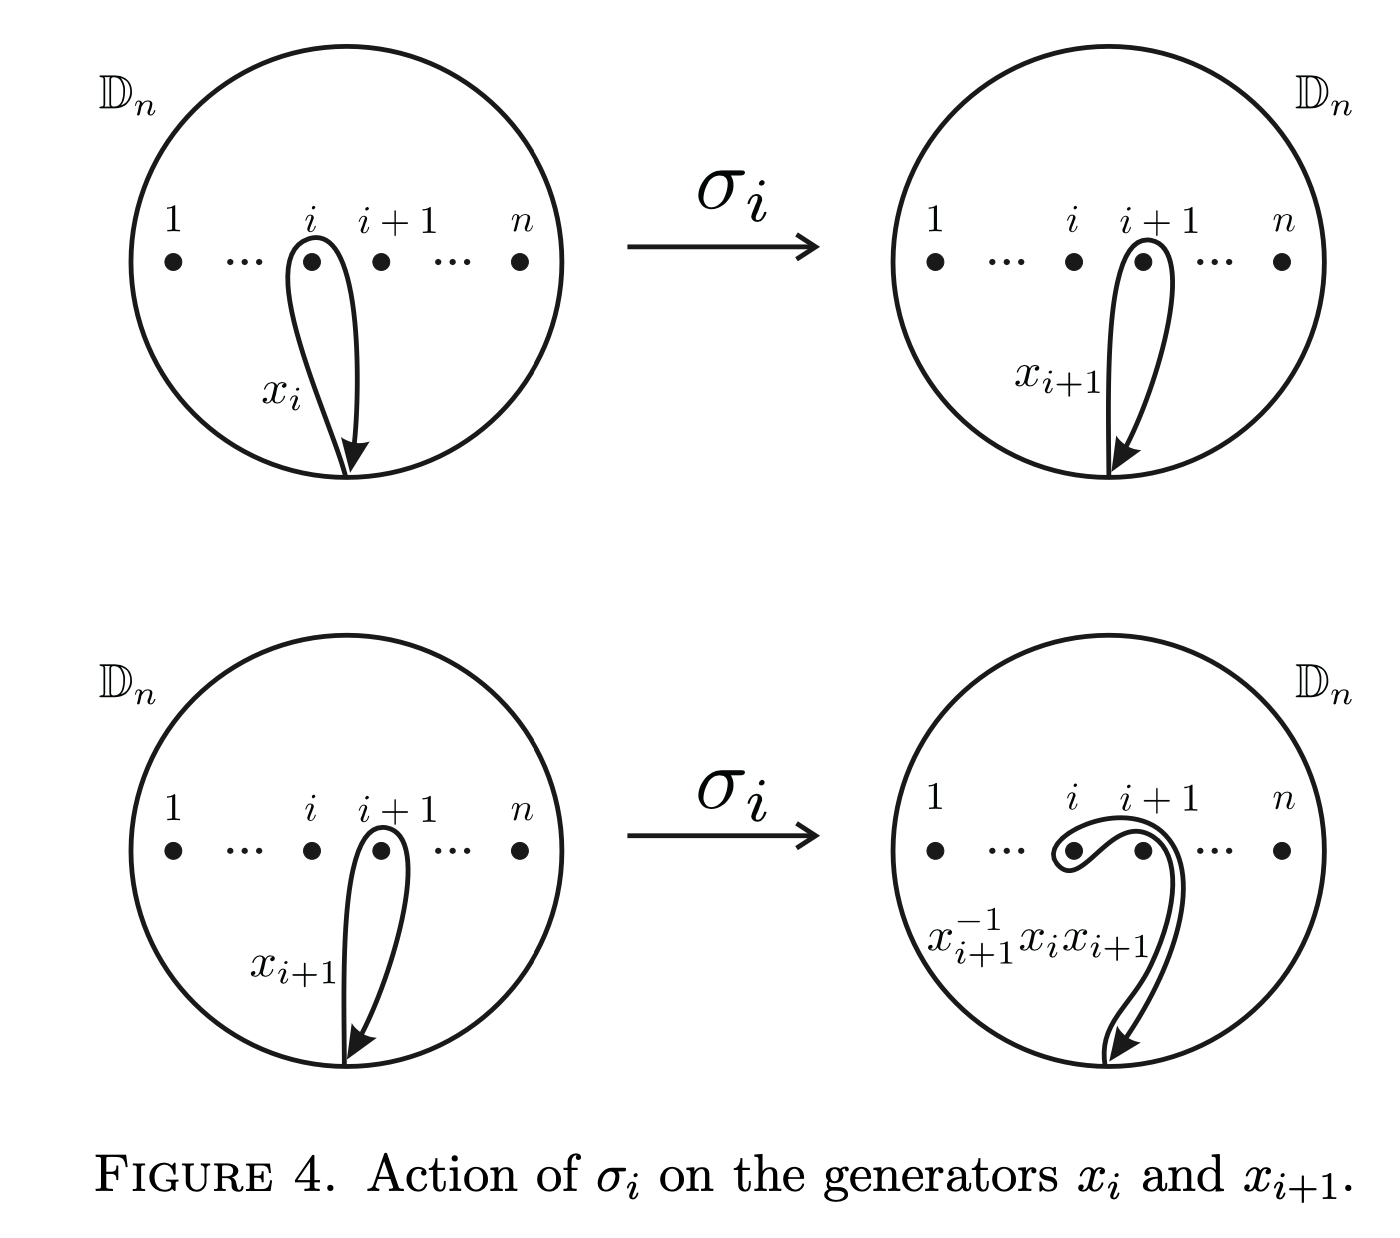
\includegraphics[width = .5\textwidth]{Gonzalez_Fig4_sigma_on_Dn.png}
%     \caption{\colorbox{red}{Gonzalez Figure 4}}\label{fig:sigma_on_Dn}
% \end{figure}

\begin{figure}[htbp]
    \centering
    \def\circleRadius{2.5cm}
\def\sep{\circleRadius*0.175}
\def\XOff{1.5*\circleRadius}
\def\YOff{-2.5*\circleRadius}

\pgfdeclarelayer{edgelayer}
\pgfdeclarelayer{nodelayer}
\pgfsetlayers{edgelayer,nodelayer,main}

\newcommand{\drawRegion}[3]{
        \begin{scope}[shift={#1}]
        \node[anchor=north west, font=\large] at (-\circleRadius, \circleRadius) {$\D_n$};

        \draw[ultra thick] (0,0) circle (\circleRadius);
        \filldraw [black] 
                (-\circleRadius + \sep,0) circle (2pt) node[above] {$1$}
                (\circleRadius - \sep,0) circle (2pt) node[above] {$n$}
                (-\sep,0) circle (2pt) node[above, yshift=.2*\sep] {$i$}
                (\sep,0) circle (2pt) node[above, yshift=.1*\sep] {$i+1$};
        \path (-\circleRadius/2,0) node {$\scalebox{1.5}{$\cdots$}$};
        \path (\circleRadius/2,0) node {$\scalebox{1.5}{$\cdots$}$};

        \ifx&#2&  % Check if #2 is empty
                % Do nothing if #2 is empty
        \else
                \draw[-latex, ultra thick] (0,-\circleRadius) .. controls #2 .. node[pos=0.1, left] {#3} (.05*\sep,-\circleRadius + 2.8452755906/2);
        \fi
        
        \filldraw [red] (0,-\circleRadius) circle (2pt);
        
        \end{scope}
}


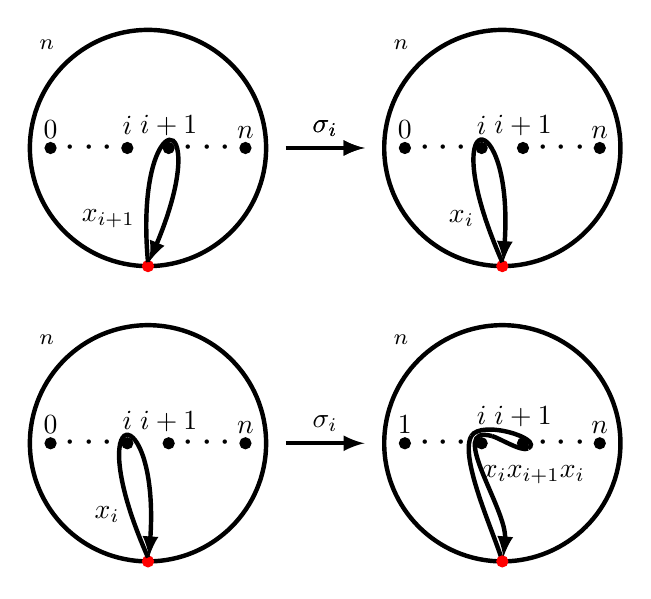
\begin{tikzpicture}
        \drawRegion{(\XOff,0)}{(-1.425*\sep-.35*\circleRadius,0.39*\circleRadius) and  (-1.425*\sep+.35*\circleRadius,0.39*\circleRadius)}{$x_i$}
        
        \draw[-latex, ultra thick] (-\XOff + \circleRadius + 0.25cm, 0) -- node[above] {$\sigma_i$} (\XOff - \circleRadius - 0.25cm, 0);
        
        \drawRegion{(-\XOff,0)}{(1.3*\sep-.35*\circleRadius,0.39*\circleRadius) and  (1.3*\sep+.35*\circleRadius,0.39*\circleRadius)}{$x_{i+1}$}
        
        \drawRegion{(-\XOff,\YOff)}{(-1.425*\sep-.35*\circleRadius,0.39*\circleRadius) and  (-1.425*\sep+.35*\circleRadius,0.39*\circleRadius)}{$x_i$}

        \draw[-latex, ultra thick] (-\XOff + \circleRadius + 0.25cm, \YOff) -- node[above] {$\sigma_i$} (\XOff - \circleRadius - 0.25cm, \YOff);
        
        % \drawRegion{(\XOff,\YOff)}{}{}

        \begin{scope}[shift={(\XOff,\YOff)}]
                \node[anchor=north west, font=\large] at (-\circleRadius, \circleRadius) {$\D_n$};
        
                \draw[ultra thick] (0,0) circle (\circleRadius);
                \filldraw [black] 
                        (-\circleRadius + \sep,0) circle (2pt) node[above] {$1$}
                        (\circleRadius - \sep,0) circle (2pt) node[above] {$n$}
                        (-\sep,0) circle (2pt) node[above, yshift=.45*\sep] {$i$}
                        (\sep,0) circle (2pt) node[above, yshift=.3*\sep] {$i+1$};
                \path (-\circleRadius/2,0) node {$\scalebox{1.5}{$\cdots$}$};
                \path (\circleRadius/2,0) node {$\scalebox{1.5}{$\cdots$}$};
        
                \filldraw [red] (0,-\circleRadius) circle (2pt);

                \begin{pgfonlayer}{nodelayer}
                        \node (0) at (-1.5*\sep,.35*\sep ) {};
                        \node (1) at (0, -\circleRadius) {};
                        \node (2) at (1.5*\sep, -1.5*\sep) {$x_i x_{i+1}\iv{x_i}$};
                        \node (3) at (1.25*\sep, -.25*\sep) {};
                        \node (4) at (-.5*\sep, .35*\sep) {};
                        \node (5) at (.05*\sep, -\circleRadius + 2.8452755906/2) {};
                \end{pgfonlayer}
                \begin{pgfonlayer}{edgelayer}
                        \draw [in=105, out=-120, looseness=0.50, ultra thick] (0.center) to (1.center);
                        \draw [in=60, out=30, looseness=0.85, ultra thick] (3.center) to (0.center);
                        \draw [in=-150, out=-15, looseness=0.50, ultra thick] (4.center) to (3.center);
                        \draw [latex-, in=165, out=85, ultra thick] (5.center) to (4.center);
                \end{pgfonlayer}

                % \foreach \point in {0,1,3,4,5} {
                %         \fill[red] (\point) circle (2pt);
                %         \node[above right] at (\point) {\point};
                % }
        \end{scope}
        
        \draw[-latex, ultra thick] (-\XOff + \circleRadius + 0.25cm, 0) -- node[above] {$\sigma_i$} (\XOff - \circleRadius - 0.25cm, 0);
\end{tikzpicture}
    \caption{The action of $\sigma_i$ on the generators $x_i$ and $x_{i+1}$ as described by \cref{eq:rho_i,eq:rho_ip1,eq:rho_j}. The image of $x_i$ under $\sigma_i$ is verified visually in \cref{fig:sigma_on_x_i}}\label{fig:sigma_on_Dn}
\end{figure}

The automorphism $\rho_\beta$ is most simply defined in terms of the action of the standard generators of $B_n$ on the generators $x_1,\dots,x_n$ of $F_n$ (visualized as loops in $\D_n$). For each $i$, it follows that
\begin{align}
    &\rho_{\sigma_i}(x_{i}) = x_{i}x_{i+1} \iv{x_{i}}, \label{eq:rho_i}\\
    &\rho_{\sigma_i}(x_{i+1}) = x_{i}, \label{eq:rho_ip1}\\
    &\rho_{\sigma_i}(x_j) = x_j, \textrm{ for } j\neq i,i-1.\label{eq:rho_j}
\end{align}
Clearly, any two loops that are separated by at least one puncture will not interact while performing $\sigma_i$. The relations for adjacent loops can be verified graphically as illustrated in \cref{fig:sigma_on_Dn,fig:sigma_on_x_i}.
\begin{figure}[htbp]
    \centering
    \def\circleRadius{2.5cm}
\def\sep{\circleRadius*0.175}
\def\XOff{1.5*\circleRadius}
\def\YOff{-2.5*\circleRadius}

\usetikzlibrary{decorations.markings}

\pgfdeclarelayer{edgelayer}
\pgfdeclarelayer{nodelayer}
\pgfsetlayers{edgelayer,nodelayer,main}

\newcommand{\drawRegion}[3]{
        \begin{scope}[shift={#1}]
        \node[anchor=north west, font=\large] at (-\circleRadius, \circleRadius) {$\D_n$};

        \draw[ultra thick] (0,0) circle (\circleRadius);
        \filldraw [black] 
                (-\circleRadius + \sep,0) circle (2pt) node[above] {$0$}
                (\circleRadius - \sep,0) circle (2pt) node[above] {$n$}
                (-\sep,0) circle (2pt) node[above, yshift=.2*\sep] {$i$}
                (\sep,0) circle (2pt) node[above, yshift=.1*\sep] {$i+1$};
        \path (-\circleRadius/2,0) node {$\scalebox{1.5}{$\cdots$}$};
        \path (\circleRadius/2,0) node {$\scalebox{1.5}{$\cdots$}$};

        \filldraw [red] (0,-\circleRadius) circle (2pt);

        \ifx&#2&  % Check if #2 is empty
                % Do nothing if #2 is empty
        \else
                \draw[-latex, ultra thick] (0,-\circleRadius + 2.8452755906/2) .. controls #2 .. node[pos=0.1, left] {#3} (.05*\sep,-\circleRadius + 2.8452755906/2);
        \fi
        \end{scope}
}

\newcommand{\drawloop}[4]{\draw[ultra thick, postaction={decorate}, decoration={markings, mark= at position 0.75 with {\arrow{latex},sloped}}, #2] (0,-\circleRadius + 2.8452755906/2) .. controls #1 .. node[pos=#4, left] {#3} (.05*\sep,-\circleRadius + 2.8452755906/2);}

\newcommand{\rdrawloop}[4]{\draw[ultra thick, postaction={decorate}, decoration={markings, mark= at position 0.25 with {\arrowreversed{latex},sloped}}, #2] (0,-\circleRadius + 2.8452755906/2) .. controls #1 .. node[pos=#4, left] {#3} (.05*\sep,-\circleRadius + 2.8452755906/2);}


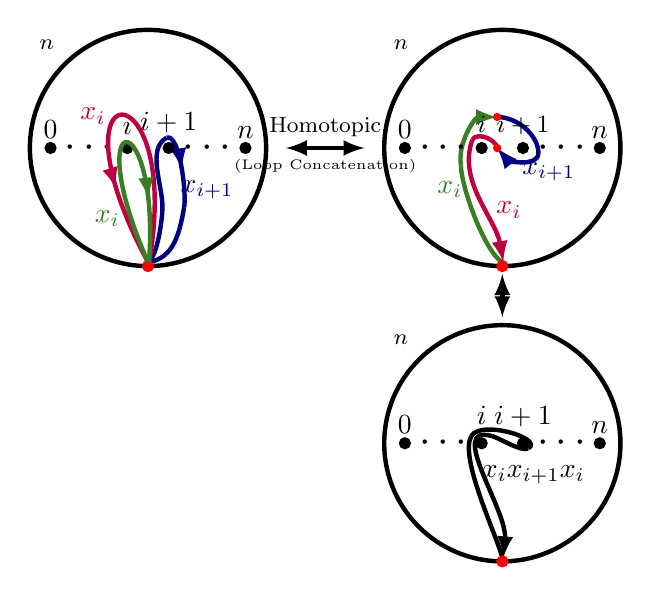
\begin{tikzpicture}
        \begin{scope}[shift={(-\XOff,0)}]
                \node[anchor=north west, font=\large] at (-\circleRadius, \circleRadius) {$\D_n$};
        
                \draw[ultra thick] (0,0) circle (\circleRadius);
                \filldraw [black] 
                        (-\circleRadius + \sep,0) circle (2pt) node[above] {$0$}
                        (\circleRadius - \sep,0) circle (2pt) node[above] {$n$}
                        (-\sep,0) circle (2pt) node[above, yshift=.2*\sep] {$i$}
                        (\sep,0) circle (2pt) node[above, yshift=.25*\sep] {$i+1$};
                \path (-\circleRadius/2,0) node {$\scalebox{1.5}{$\cdots$}$};
                \path (\circleRadius/2,0) node {$\scalebox{1.5}{$\cdots$}$};
        
                \filldraw [red] (0,-\circleRadius) circle (2pt);

                \begin{pgfonlayer}{nodelayer}
                        \node (0) at (.7*\sep,-.5*\circleRadius ) {};
                        \node (1) at (0, -\circleRadius + 2.8452755906/2) {};
                        \node (2) at (.5*\circleRadius, -2*\sep) {$\color{NavyBlue} x_{i+1}$};
                        \node (3) at (.9*\sep, .5*\sep) {};
                        \node (4) at (1.75*\sep, -.5*\circleRadius) {};
                        \node (5) at (.05*\sep, -\circleRadius + 2.8452755906/2) {};
                \end{pgfonlayer}
                \begin{pgfonlayer}{edgelayer}
                        \draw [in=30, out=-90, looseness=0.50, ultra thick, NavyBlue] (0.center) to (1.center);
                        \draw [in=90, out=-150, looseness=0.85, ultra thick, NavyBlue] (3.center) to (0.center);
                        \draw [in=20, out=80, looseness=0.50, ultra thick, NavyBlue, postaction={decorate}, decoration={markings, mark= at position .5 with {\arrowreversed{latex},sloped}}] (4.center) to (3.center);
                        \draw [in=-100, out=10, ultra thick, NavyBlue] (5.center) to (4.center);
                \end{pgfonlayer}
                
                % \foreach \point in {0,1,3,4,5} {
                %         \fill[red] (\point) circle (2pt);
                %         \node[above right] at (\point) {\point};
                % }

                \rdrawloop{(-1.4*\sep-.65*\circleRadius,0.7*\circleRadius) and  (-1.4*\sep+.55*\circleRadius,0.7*\circleRadius)}{purple}{$\iv{x_i}$}{.45}

                \drawloop{(-1.4*\sep-.35*\circleRadius,0.39*\circleRadius) and  (-1.4*\sep+.35*\circleRadius,0.39*\circleRadius)}{OliveGreen}{$x_i$}{.1}

        \end{scope}

        \begin{scope}[shift={(\XOff,0)}]
                \node[anchor=north west, font=\large] at (-\circleRadius, \circleRadius) {$\D_n$};
        
                \draw[ultra thick] (0,0) circle (\circleRadius);
                \filldraw [black] 
                        (-\circleRadius + \sep,0) circle (2pt) node[above] {$0$}
                        (\circleRadius - \sep,0) circle (2pt) node[above] {$n$}
                        (-\sep,0) circle (2pt) node[above, yshift=.3*\sep] {\small$i$}
                        (\sep,0) circle (2pt) node[above, xshift=0*\sep, yshift=.15*\sep] {\small$i+1$};
                \path (-\circleRadius/2,0) node {$\scalebox{1.5}{$\cdots$}$};
                \path (\circleRadius/2,0) node {$\scalebox{1.5}{$\cdots$}$};
        
                \filldraw [red] (0,-\circleRadius) circle (2pt);
                
                \begin{scope}[shift={(-.25*\sep,0)}]
                                \begin{pgfonlayer}{nodelayer}
                                \node (0) at (-1.75*\sep,-.15*\circleRadius ) {};
                                \node (1) at (.25*\sep, -\circleRadius + 2.8452755906/2) {};
                                % \node (2) at (.5*\circleRadius, -2*\sep) {$x_i x_{i+1}\iv{x_i}$};
                                \node (3) at (0*\sep, 1.5*\sep) {};
                                \node (4) at (2*\sep, -.05*\circleRadius) {};
                                \node (5) at (0*\sep, 0*\circleRadius) {};
                                \node (6) at (-1.2*\sep, .4*\sep) {};
                                \node (7) at (.3*\sep, -\circleRadius + 2.8452755906/2) {};

                                \node (ip1) at (2.5*\sep, -1.15*\sep) {$\color{NavyBlue} x_{i+1}$};
                                \node (i) at (-.4*\circleRadius, -2*\sep) {$\color{OliveGreen} x_{i}$};
                                \node (iiv) at (.1*\circleRadius, -3*\sep) {$\color{purple} \iv{x_{i}}$};
                        \end{pgfonlayer}
                        \begin{pgfonlayer}{edgelayer}
                                \draw [in=150, out=-90, looseness=0.50, ultra thick, OliveGreen] (0.center) to (1.center);
                                \draw [latex-, in=100, out=180, looseness=0.95, ultra thick, OliveGreen] (3.center) to (0.center);
                                \draw [in=0, out=90, looseness=0.9, ultra thick, NavyBlue] (4.center) to (3.center);
                                \draw [latex-, in=-100, out=-50, looseness=.9, ultra thick, NavyBlue] (5.center) to (4.center);
                                \draw [in=60, out=100, looseness=.9, ultra thick, purple] (5.center) to (6.center);
                                \draw [-latex, in=100, out=-110, looseness=.9, ultra thick, purple] (6.center) to (7.center);
                        \end{pgfonlayer}
                \end{scope}
                
                \foreach \point in {3,5} {
                                \fill[red] (\point) circle (1.5pt);
                                % \node[above right] at (\point) {\point};
                        }

                % \foreach \point in {0,1,3,4,5,6,7} {
                %         \fill[red] (\point) circle (1.5pt);
                %         \node[above right] at (\point) {\point};
                % }
        \end{scope}

        \begin{scope}[shift={(\XOff,\YOff)}]
                \node[anchor=north west, font=\large] at (-\circleRadius, \circleRadius) {$\D_n$};
        
                \draw[ultra thick] (0,0) circle (\circleRadius);
                \filldraw [black] 
                        (-\circleRadius + \sep,0) circle (2pt) node[above] {$0$}
                        (\circleRadius - \sep,0) circle (2pt) node[above] {$n$}
                        (-\sep,0) circle (2pt) node[above, yshift=.45*\sep] {$i$}
                        (\sep,0) circle (2pt) node[above, yshift=.3*\sep] {$i+1$};
                \path (-\circleRadius/2,0) node {$\scalebox{1.5}{$\cdots$}$};
                \path (\circleRadius/2,0) node {$\scalebox{1.5}{$\cdots$}$};
        
                \filldraw [red] (0,-\circleRadius) circle (2pt);

                \begin{pgfonlayer}{nodelayer}
                        \node (0) at (-1.5*\sep,.35*\sep ) {};
                        \node (1) at (0, -\circleRadius + 2.8452755906/2) {};
                        \node (2) at (1.5*\sep, -1.5*\sep) {$x_i x_{i+1}\iv{x_i}$};
                        \node (3) at (1.25*\sep, -.25*\sep) {};
                        \node (4) at (-.5*\sep, .35*\sep) {};
                        \node (5) at (.05*\sep, -\circleRadius + 2.8452755906/2) {};
                \end{pgfonlayer}
                \begin{pgfonlayer}{edgelayer}
                        \draw [in=105, out=-120, looseness=0.50, ultra thick] (0.center) to (1.center);
                        \draw [in=60, out=30, looseness=0.85, ultra thick] (3.center) to (0.center);
                        \draw [in=-150, out=-15, looseness=0.50, ultra thick] (4.center) to (3.center);
                        \draw [latex-, in=165, out=85, ultra thick] (5.center) to (4.center);
                \end{pgfonlayer}

        \end{scope}
        
        \draw[latex-latex, ultra thick] (-\XOff + \circleRadius + 0.25cm, 0) -- node[above] {\footnotesize Homotopic} node[below] {\tiny (Loop Concatenation)} (\XOff - \circleRadius - 0.25cm, 0);
        
        \draw[latex-latex, ultra thick] (\XOff, -\circleRadius - 0.1cm) -- (\XOff, \YOff+\circleRadius + 0.1cm);
\end{tikzpicture}
    \caption{Up to homotopy, the product $x_i x_{i+1} \iv{x_i}$ is visualized as the concatenation of the loops $x_i,x_{i+1},\iv{x_i}\in\pi_1(\D_n)$. In the top right diagram, small red dots are used indicate the (homotopically deformed) points of concatenation.}\label{fig:sigma_on_x_i}
\end{figure}

For any $\sigma_i$, $\rho_{\iv{\sigma_i}}$ is well-defined. It follows that for any braid $\beta\in B_n$, we can decompose $\rho_\beta$ the composition of the automorphisms of the standard generators $\sigma_1,\dots,\sigma_{n-1}$ and their inverses that make up $\beta$. 

Notice that for any $\sigma_i$, $\rho_{\sigma_i}(x_1\cdots x_n) = x_1\cdots x_n$. This is because the loop $x_1\cdots x_n$ in $\D_n$, encompassing all holes, is parallel to the boundary $\partial\D_n$. Thus, the action of $\sigma_i$ on $x_1\cdots x_n$ is trivial does not affect the structure of the loop up to isotopy. More generally, this implies that $\rho_\beta(x_1\cdots x_n) = x_1\cdots x_n$ for any $\beta\in B_n$. Paired with the observation that every generator is conjugate to another, Artin~\cite{Artin1947} showed that this is a necessary and sufficient condition for $\rho_\beta$ to be an automorphism of $F_n$.

\begin{theorem}\label{thm:autFn}
    An automorphism $f\in\aut{F_n}$ is equal to $\rho_\beta$ for some $\beta\in B_n$ if and only if
    \begin{enumerate}
        \item $f(x_i)$ is a conjugate of some $x_j$ for every $i\in\left\{ 1,\dots,n \right\}$, and
        \item $f(x_1\cdots x_n) = x_1\cdots x_n$.
    \end{enumerate}
\end{theorem}

In this interpretation of the braid group, we can express $B_n$ in terms of the standard generators:
\begin{equation}\label{eq:BnGenYangBaxter}
    B_n = \left\langle \sigma_1,\dots,\sigma_{n-1} \;\middle|\;
    \begin{aligned}
        \sigma_i\sigma_j &= \sigma_j\sigma_i, & |i-j|&>1 \\
        \sigma_i\sigma_{i+1}\sigma_i &= \sigma_{i+1}\sigma_i\sigma_{i+1}, & |i-j|&=1
    \end{aligned}
    \right\rangle.
\end{equation}
The first condition that the standard generators commute if $|i-j|>1$ is easily verified by thinking about the action of the generators on $\pi_1(\D_n)$ as in \cref{fig:sigma_on_Dn} and as automorphisms in \cref{eq:rho_j}. This follows from the fact that if punctures $i$ and $j$ are non-adjacent, then the actions of $\sigma_i$ and $\sigma_j$ are mutually exclusive and thus commutative. The second condition on the standard generators is most easily verified in \cref{fig:YB_criterion_verification} by looking at the corresponding braids in $\R\times[0,1]$ (here, the distinction between $\R$ and $\C$ is only a matter of choosing to show the starting and ending complex planes in traditional braid visualizations).
\begin{figure}[htbp]
    \centering
    % 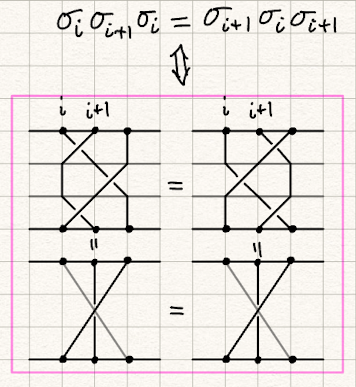
\includegraphics[width = .5\textwidth]{sketch_YB_citerion_verification.png}
    \def\sep{3cm}
\def\offset{.875cm}
\def\customGap{.125cm}

\begin{tikzpicture}[
    braid/.cd,
    crossing convention=under,
    anchor=center,
    every strand/.style={ultra thick},
    strand 1/.style={red},
    strand 2/.style={blue},
    strand 3/.style={green},
    ]

    \coordinate (center) at (0,0);
    
    \pic (121) at (-1.5*\sep,0) {braid={s_1 s_2 s_1}} node[below, at=(121-2-e)] {$\sigma_1\sigma_2\sigma_1$};
    \pic (212) at (1.5*\sep,0) {braid={s_2 s_1 s_2}} node[below, at=(212-2-e)] {$\sigma_2\sigma_1\sigma_2$};
    \pic[braid/.cd,
        gap=0.015,
        control factor=0,
        nudge factor=0,
        width=2cm,
        crossing height=3cm,
        strand 1/.style={blue},
        strand 2/.style={green},
    ] (eq1) at (-.5*\sep,0) {braid={s_1}};
    \pic[braid/.cd,
        gap=0.015,
        control factor=0,
        nudge factor=0,
        width=2cm,
        crossing height=3cm,
        strand 1/.style={blue},
        strand 2/.style={green},
    ] (eq2) at (.5*\sep,0) {braid={s_1}};

    \begin{scope}[on background layer]
        \draw[ultra thick, red] ($(eq1-1-s) + (-.225cm,-\offset)$) -- ($(eq1-2-s) + (.225cm,-\offset)$);
        \draw[ultra thick, red] ($(eq2-2-e) + (-.225cm,\offset)$) -- ($(eq2-1-e) + (.225cm,\offset)$);        
        \foreach \i in {1,2} {
            \foreach \j in {1,2}{
                \draw[line width=\customGap, white] ($(eq\i-\j-s) - (0,.25cm)$) -- ($(eq\i-\j-e) + (0,.25cm)$);
            }
        }
    \end{scope}

    \draw[latex-latex, out=70, in=110, looseness=.75, line width=1.2pt] ($(eq1-1-s) + (1cm,.1cm)$) to node[pos=.5,above, font=\footnotesize] {Reidemeister type-III move} ($(eq2-2-s) + (-1cm,.1cm)$);

    \node at ($(121)!.5!(eq1)$) {$=$};
    \node at ($(eq1)!.5!(eq2)$) {$=$};
    \node at ($(eq2)!.5!(212)$) {$=$};
\end{tikzpicture}
    \caption{Graphical verification of \cref{eq:BnGenYangBaxter}. All of the above braids are equivalent up to homotopy. The transformation between the middle two braid diagrams is known as a Reidmeister type-III move, in which the red strand (or string in the context of knot theory) is moved completely under the crossing of the blue and green strands. In these middle two diagrams, the red strand is slightly translucent to indicate that it is behind all other strands in the diagram.}\label{fig:YB_criterion_verification}
\end{figure}

\section[One-dimensional representations of $B_n$]{One-dimensional representations of $\mathbf{B_n}$}
A straightforward nontrivial representation of the braid is defined on the standard generators of $B_n$ and is given by \cite{Deshmukh}:
\begin{align}
    p_\theta: B_n&\to \C_{\size{z}=1} \\
    \sigma_i &\mapsto e^{i\theta},
\end{align}
for $\theta\in\R$. Clearly, $p_\theta$ is a homomorphism, and it is unitary because
\begin{equation}
    {p_\theta(\sigma_i)}^\dagger = {\left( e^{i\theta} \right)}^\dagger = e^{-i\theta} = \iv{\left( e^{i\theta} \right)} = \iv{p_\theta(\sigma_i)},
\end{equation}
where $^\dagger$ denotes the conjugate transpose of a matrix. Notice that with a choice of $\theta=2\pi n$ for $n\in\Z$, we recover the trivial representation of $B_n$. Similarly, $p_{\pi n}$ is a restriction of the sign representation of $S_n$, where the sign of a permutation is defined as the parity of the number of transpositions in its decomposition into a product of transpositions.

% The degree 1 representations of $B_n$ will be revisited in \cref{sec:Anyons}.

\section{The Burau Representation}
In the previous section, we defined a representation of the braid group $B_n$ as automorphisms of the free group $F_n$. This representation is clearly nonabelian. Likewise, the Artin generators of $B_n$ are nonabelian. Suppose we wish to abelianize the braid group. The details of the abelianization of $B_n$ would require a quotient by the commutator $\left[ a,b \right]=ab\iv{a}\iv{b}$.

Sparing the details, let $B_{n,ab} = B_n/\left[ B_n,B_n \right]$ be the abelianization of $B_n$, where $\left[ B_n,B_n \right]=\left\{ \left[ \beta_1,\beta_2 \right]\st\beta_1,\beta_2\in B_n \right\}$ is the commutator subgroup of $B_n$. Then, under the representation $\rho$ from \cref{sec:Aut_Fn}, the abelianization of \cref{eq:rho_i,eq:rho_ip1,eq:rho_j} become
\begin{align}
    x_i &\xmapsto{\sigma_i} \cancel{x_i} + x_{i+1} - \cancel{x_i} = x_{i+1} = \rho_{\iv{\sigma_i}}(x_i), \\
    x_{i+1} &\xmapsto{\sigma_i} x_i, \\
    x_j &\xmapsto{\sigma_i} x_j, \textrm{ for } j\neq i,i-1,
\end{align}
for each $i$. Thus, the generator $\sigma_i=\iv{\sigma_i}$, and corresponds to a transposition permutation in the symmetric group $S_n$. It follows that $B_{n,ab}\iso S_n$. In this current construction, the abelianization of the braid group results in a loss of complexity. This raises the question whether there exists such a reframing of the braid group that allows an abelian operation on the free generators while preserving the inequivalence of the Artin generators with their inverses.

First, we define a topological space that will aid in the desired construction.
\begin{definition}
    Let $X$ be a topological space. A \textit{covering} of $X$ is a space $\widetilde{X}$ together with a continuous map $p:\widetilde{X}\to X$ such that, for every $x\in X$, there exists a path-connected open neighborhood $U$ containing $x$ such that $\iv{p}(U)$ is a disjoint union of open sets in $\widetilde{X}$ where each component of $\iv{p}(U)$ is mapped homeomorphically onto $U$ by $p$. Each component of $\iv{p}(U)$ is called a \textit{sheet} of the covering, where the $i$-th sheet is denoted by $\sheet{X}{i}$, and total the number of sheets in $\iv{p}(U)$ is called the \textit{degree} of the covering.
\end{definition}

\begin{example}
    One of the simplest examples of a covering space is the covering of the circle $S^1$ by the real line by the parameterization map $p:\R\to S^1$ defined by $p(t)=\left( \cos t,\sin t \right)$. Clearly, there are infinitely many sheets in this covering.
\end{example}

\begin{example}
    A similar example is the covering of the circle $S^1$ through $p:\left[ 0,1 \right]\to S^1$ defined by $p(t) = e^{2\pi it}$. This defines a one-degree covering of $S^1$. If we instead let our domain be $\left[ 0,2 \right]$, then we have a two-degree covering of $S^1$.
\end{example}

With this topological tool, we construct a countably infinite-degree covering of the punctured disk $\D_n$, denoted $\widetilde{\D}_n$, which can be visualized as an infinite stack of copies of $\D_n$, with a slight modification to be explained shortly. Let $\sheet{\D}{n,i}$ denote the $i$-th sheet of $\widetilde{\D}_n$, and consider the base sheet our covering to be $\sheet{\D}{n,0}$.

We start this construction with a countably infinite stack of copies of $\D_n$. Then, for every $i\in\Z$, for each of the $n$ punctures on $\sheet{\D}{n,i}$, apply a cut from the hole to some point on the boundary of $\sheet{\D}{n,i}$, as illustrated in \cref{fig:D3_cuts} for the case when $n=3$. Each cut results in two edges, which will be referred to as the left edge and the right edge. Through a homeomorphic deformation, connect the left edge of $\sheet{\D}{n,i}$ to the corresponding right edge of $\sheet{\D}{n,i+1}$, and the right edge of $\sheet{\D}{n,i}$ to the left edge of $\sheet{\D}{n,i-1}$, for every cut on every sheet.

\begin{figure}[htbp]
    \centering
    % 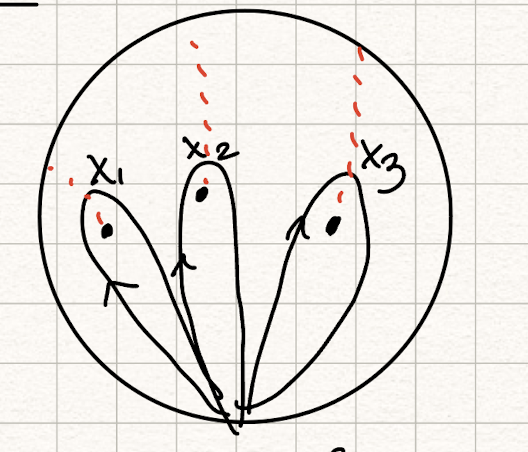
\includegraphics[width=.3\textwidth]{D3_cuts.png}
    % Suggested circle radius >= 3 cm
\usetikzlibrary{
        math,
        calc,
        % decorations.markings,
}

\def\circleRadius{3cm}
\def\sep{\circleRadius*0.175}
% \def\Off{.6}
% \def\eSep{.0005*\circleRadius}
% \def\cSep{1.2*\eSep}
\def\aSep{5} % degrees
\def\lA{130}
\def\cA{90}
\def\rA{50}

\begin{tikzpicture}[
] 
        \node[anchor=north west, font=\Large] at ({-1.15*\circleRadius}, {1.05*\circleRadius}) {$\sheet{\D}{n,i}$};

        \draw[ultra thick] (0,0) circle (\circleRadius);

        \tikzmath{
                coordinate \l, \r, \p, \b, \lI, \lO; real \aL, \aR;
                \aL1 = \lA+\aSep;
                \aR1 = \lA-\aSep;
                \aL2 = \cA+\aSep;
                \aR2 = \cA-\aSep;
                \aL3 = \rA+\aSep;
                \aR3 = \rA-\aSep;
                %
                \b = (0,-\circleRadius);
                \p1 = (-.5*\circleRadius,0);
                \p2 = (0,0);
                \p3 = (.5*\circleRadius,0);
                \l1 = (\aL1:\circleRadius);
                \r1 = (\aR1:\circleRadius);
                \l2 = (\aL2:\circleRadius);
                \r2 = (\aR2:\circleRadius);
                \l3 = (\aL3:\circleRadius);
                \r3 = (\aR3:\circleRadius);
                %
        %         Alternate method with cartesian coordinates
        %         \l1 = ({-(\Off + \eSep)*\circleRadius},{sqrt(1-(\Off + \eSep)^2) * \circleRadius});
        %         \l2 = (-\cSep*\circleRadius,{sqrt(1-(\cSep)^2) * \circleRadius});
        %         \l3 = ({(\Off - \eSep)*\circleRadius},{sqrt(1-(\Off - \eSep)^2) * \circleRadius});
        %         \r1 = ({-(\Off - \eSep)*\circleRadius},{sqrt(1-(\Off - \eSep)^2) * \circleRadius});
        %         \r2 = (\cSep*\circleRadius,{sqrt(1-(\cSep)^2) * \circleRadius});
        %         \r3 = ({(\Off + \eSep)*\circleRadius},{sqrt(1-(\Off + \eSep)^2) * \circleRadius});
        }
        
        % \foreach \i in {1,2,3} {
        %         \draw[white, line width=2pt] (\r\i) arc (atan2(\ry\i,\rx\i):atan2(\ly\i,\lx\i):\circleRadius);
        % }

        \foreach \i in {1,2,3} {
                \draw[white, line width=2pt] (\r\i) arc (\aR\i:\aL\i:\circleRadius);
        }

        % Alternate method with nodes
        % \node (l1) at ({\lA+\aSep}:\circleRadius) {};
        % \node (r1) at ({\lA-\aSep}:\circleRadius) {};
        % 
        % \node (l2) at ({\cA+\aSep}:\circleRadius) {};
        % \node (r2) at ({\cA-\aSep}:\circleRadius) {};
        % 
        % \node (l3) at ({\rA+\aSep}:\circleRadius) {};
        % \node (r3) at ({\rA-\aSep}:\circleRadius) {};

        \foreach \i in {1,2,3} {
                \coordinate (lI\i) at ($(\p\i)!0.5!(\l\i)$);
                \coordinate (lO\i) at ($(\p\i)!0.5!(\r\i)$);

                \fill[cyan] (\l\i) circle (.75pt);
                \fill[purple] (\r\i) circle (.75pt);
        }

        \node at (\l2) [left, yshift=-.3*\circleRadius, xshift=.04*\circleRadius, cyan] {$\substack{\textrm{Left} \\ \textrm{Edge}}$};
        \node at (\r2) [right, yshift=-.3*\circleRadius, xshift=-.04*\circleRadius, purple] {$\substack{\textrm{Right} \\ \textrm{Edge}}$};

        \draw [out=135, in=-140, looseness=.65, line width= 1.4, decoration={markings, mark= at position 0.6 with {\arrow{latex},sloped}}, postaction={decorate}] (\b) to (lI1);
        

        \draw [out=80, in=-170, looseness=.65, line width= 1.4, decoration={markings, mark= at position 0.6 with {\arrowreversed{latex},sloped}}, postaction={decorate}] (\b) to (lI3);

        \draw [out=110, in=-110, looseness=0, ultra thick, cyan] (\p1) to (\l1);
        \draw [out=110, in=-110, looseness=0, ultra thick, cyan] (\p2) to (\l2);
        \draw [out=110, in=-110, looseness=0, ultra thick, cyan] (\p3) to (\l3);
        
        \draw [out=80, in=-80, looseness=0, ultra thick, purple] (\p1) to (\r1);
        \draw [out=80, in=-80, looseness=0, ultra thick, purple] (\p2) to (\r2);
        \draw [out=80, in=-80, looseness=0, ultra thick, purple] (\p3) to (\r3);

        \foreach \i in {1,2,3} {
                \fill[black] (\p\i) circle (2pt);
                \node[above, yshift=-.15*\sep, xshift=.45*\sep] at (\p\i) {$\i$};
        }

        % base point for loop/arrow
        \filldraw [red] (\b) circle (2pt) node[below] {$t^i\zeta$};
\end{tikzpicture}

    \caption{
        % In the case of $\D_3$, this figure demonstrates how the cuts are applied across each of the three punctures for each sheet in the covering $\widetilde{\D}_3$. The power of $t$ in the base point label $t^j\zeta$ indicates that we are on the $j$-th sheet of the covering.
        For the covering of $\D_3$, we observe the $i$-th sheet of $\widetilde{\D}_3$ with the cuts applied across each of the three punctures. The base point of the loop is indicated by the red dot, and labelled as $t^i\zeta$. The power of $t$ indicates that we are on the $i$-th sheet of the covering. The portions of three different loops are drawn to illustrate the behavior of loops as they pass through various edges on $\sheet{\D}{3,i}$. The loop that would traditionally be $x_1$ is labeled by $t^i x_1$ to indicate that it's starting on the $i$-th sheet. When it passes through the left edge corresponding to this puncture labeled with a 1, it traverses up to the sheet $\sheet{\D}{3,i+1}$ and ends at base point $t^{i+1}\zeta$. Similarly, the loop that starts on $\sheet{\D}{3,i-1}$ and passes through the left edge of puncture 2 ends up coming out of the right edge of puncture 2 on $\sheet{\D}{3,i}$ and ends at the base point $t^i\zeta$. This loop is labeled by the starting sheet, so it is $t^{i-1}x_2$. Finally, the loop that starts on $\sheet{\D}{3,i+1}$ and passes through the right edge of puncture 3 ends up coming out of the left edge of puncture 3 on $\sheet{\D}{3,i}$. This loop is labeled by $-t^{i}x_3$ since it is the inverse of $t^i x_3$, with the negative sign indicating that the loop direction is reversed.
    }\label{fig:D3_cuts}
\end{figure}

Now, viewing a single sheet, say $\sheet{\D}{n,0}$, from above, when a loop with base point $\tilde{\zeta}_0$ passes through a cut from the left, it traverses up to the next sheet, and ends at the base point $\tilde{\zeta}_1$. Similarly, a loop passing through a cut from the right ends at the base point $\tilde{\zeta}_{-1}$, on the sheet $\sheet{\D}{n,-1}$ below $\sheet{\D}{n,0}$. To keep track of the various loops, we use a free parameter $t$. For example, a loop $\gamma$ that starts on $\sheet{\D}{n,j}$ would be written $t^j \gamma$, for $j\in\Z$. Notice that the substitution of a complex number for the free parameter $t$ results in a possibly finite degree covering. As an example, if we set $t$ to an $n$-th root of unity, then we obtain an $n$-th degree covering of $\D_n$. For the purposes of this construction, we will keep $t$ as a free parameter for now.{ }\cref{fig:D3_cuts} demonstrates how loops interact with the cuts on different sheets. The following example describes the action of the standard generators of $B_3$ on the covering space $\widetilde{\D}_3$.

\begin{example}\label{ex:Burau_D3}
    Consider the case when $n=3$. Then we have the corresponding covering space $\widetilde{\D}_3$ of $\D_3$. See \cref{fig:D3_cuts} for the view of a single sheet with various loops interacting with the cuts on the sheet. The actions of the standard generators of $B_3$ in $\pi_1(\D_3)$ are known, and can be visually understood in \cref{fig:sigma_on_Dn}. In the context of the covering space $\widetilde{\D}_3$, the action of the generators $\sigma_1$ and $\sigma_2$ is observed by reducing the visualization to only the base points on each sheet and the loops themselves. This can be seen in \cref{fig:Burau_D3} for the case of $\sigma_1$.
    
    \begin{figure}[h!]
        \centering
        % 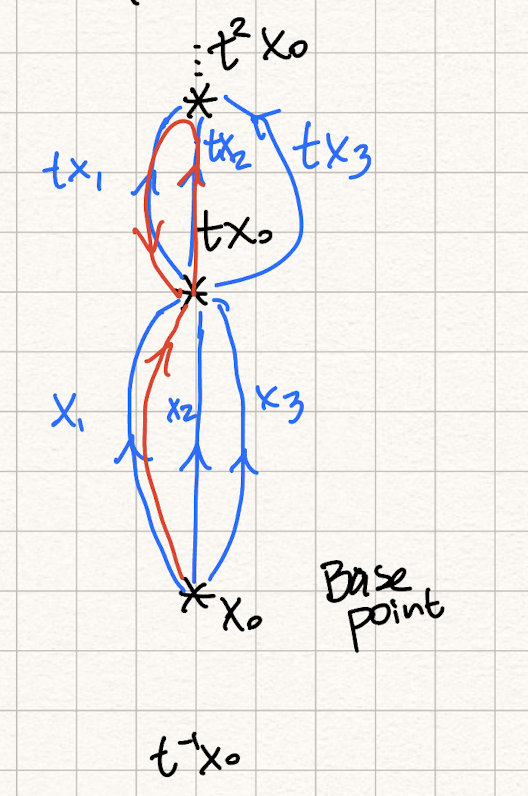
\includegraphics[width = .3\textwidth]{Burau_D3.png}
        
%
\def\circleRadius{1.5cm}
\def\sep{\circleRadius*0.175}
\def\aSep{5} % degrees
\def\lA{130}
\def\cA{90}
\def\rA{50}
%

\def\vSep{3*\circleRadius}
\def\lw{1.25pt}

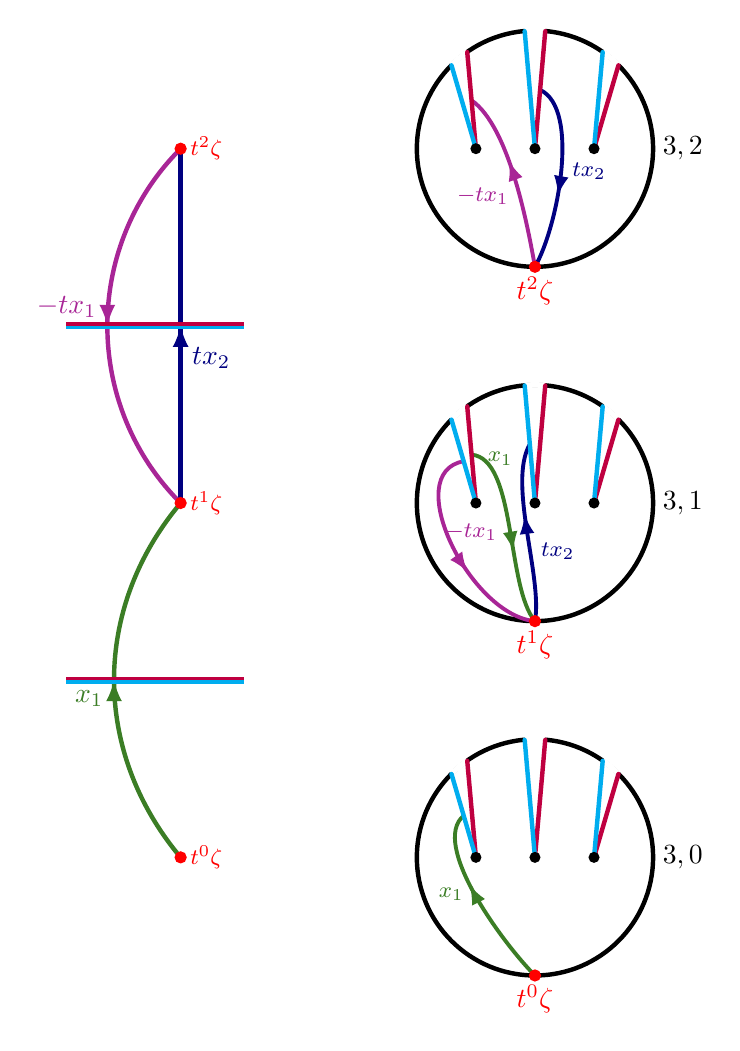
\begin{tikzpicture}[
] 

        \coordinate (t0) at (0,-\vSep);
        \coordinate (t1) at (0,0);
        \coordinate (t2) at (0,\vSep);

        % \coordinate (x1) at (-1cm,.5*\vSep);
        % \coordinate (t1x1) at (-1cm,1.5*\vSep);
        % \coordinate (x2) at (0,.5*\vSep);
        % \coordinate (x3) at (1cm,.5*\vSep);

        \draw[out=130, in=-130, ultra thick, decoration={markings, mark= at position 0.5 with {\arrow{latex},sloped}}, postaction={decorate}, OliveGreen] (t0) to node[left, pos=.45] {$x_1$} (t1);
        \draw[out=90, in=-90, ultra thick, decoration={markings, mark= at position 0.5 with {\arrow{latex},sloped}}, postaction={decorate}, NavyBlue] (t1) to node[right, pos=.4] {$tx_2$} (t2);
        \draw[out=-135, in=135, ultra thick, decoration={markings, mark= at position 0.5 with {\arrow{latex},sloped}}, postaction={decorate}, Mulberry] (t2) to node[left, pos=.45] {$-tx_1$} (t1);

        \foreach \i in {0,...,2} {
                \filldraw [red] (t\i) circle (2pt) node[right] {\footnotesize $t^\i\zeta$};
        }

        \begin{scope}[shift={(3*\circleRadius,-\vSep)}]
                \node[right] at ({1*\circleRadius}, {0*\circleRadius}) {$\sheet{\D}{3,0}$};

                \draw[ultra thick] (0,0) circle (\circleRadius);

                \tikzmath{
                        coordinate \l, \r, \p, \b; real \aL, \aR;
                        \aL1 = \lA+\aSep;
                        \aR1 = \lA-\aSep;
                        \aL2 = \cA+\aSep;
                        \aR2 = \cA-\aSep;
                        \aL3 = \rA+\aSep;
                        \aR3 = \rA-\aSep;
                        %
                        \b = (0,-\circleRadius);
                        \p1 = (-.5*\circleRadius,0);
                        \p2 = (0,0);
                        \p3 = (.5*\circleRadius,0);
                        \l1 = (\aL1:\circleRadius);
                        \r1 = (\aR1:\circleRadius);
                        \l2 = (\aL2:\circleRadius);
                        \r2 = (\aR2:\circleRadius);
                        \l3 = (\aL3:\circleRadius);
                        \r3 = (\aR3:\circleRadius);
                }

                \foreach \i in {1,2,3} {
                        \draw[white, line width=2pt] (\r\i) arc (\aR\i:\aL\i:\circleRadius);
                }

                \foreach \i in {1,2,3} {
                        \coordinate (lI\i) at ($(\p\i)!0.5!(\l\i)$);
                        \coordinate (lO\i) at ($(\p\i)!0.5!(\r\i)$);

                        \fill[cyan] (\l\i) circle (.75pt);
                        \fill[purple] (\r\i) circle (.75pt);
                }

                \draw [out=135, in=-140, looseness=.65, line width= 1.4, decoration={markings, mark= at position 0.6 with {\arrow{latex},sloped}}, postaction={decorate}, OliveGreen] (\b) to node[left, pos=.5] {\footnotesize$x_1$} (lI1);
                
                % \draw [out=80, in=-45, looseness=.65, line width= 1.4, decoration={markings, mark= at position 0.4 with {\arrowreversed{latex},sloped}}, postaction={decorate}] (\b) to (lO2);
                
                % \draw [out=25, in=-150, looseness=.65, line width= 1.4, decoration={markings, mark= at position 0.5 with {\arrowreversed{latex},sloped}}, postaction={decorate}] (\b) to (lI3);

                % \node at (-.7*\circleRadius, -.35*\circleRadius) {$x_1$};
                % \node at (-.05*\circleRadius, -.2*\circleRadius) {$t^{i-1} x_2$};
                % \node at (.475*\circleRadius, -.5*\circleRadius) {$-t^{i+1} x_3$};

                \foreach \i in {1,2,3} {
                        \draw [out=80, in=-80, looseness=0, ultra thick, purple] (\p\i) to (\r\i);
                        \draw [out=110, in=-110, looseness=0, ultra thick, cyan] (\p\i) to (\l\i);

                        \fill[black] (\p\i) circle (2pt);
                        % \node[above, yshift=-.7*\sep, xshift=.75*\sep] at (\p\i) {$\i$};
                }

                % base point for loop/arrow
                \filldraw [red] (\b) circle (2pt) node[below] {$t^0\zeta$};
        \end{scope}

        \begin{scope}[shift={(3*\circleRadius,0)}]
                \node[right] at ({1*\circleRadius}, {0*\circleRadius}) {$\sheet{\D}{3,1}$};

                \draw[ultra thick] (0,0) circle (\circleRadius);

                \tikzmath{
                        coordinate \l, \r, \p, \b; real \aL, \aR;
                        \aL1 = \lA+\aSep;
                        \aR1 = \lA-\aSep;
                        \aL2 = \cA+\aSep;
                        \aR2 = \cA-\aSep;
                        \aL3 = \rA+\aSep;
                        \aR3 = \rA-\aSep;
                        %
                        \b = (0,-\circleRadius);
                        \p1 = (-.5*\circleRadius,0);
                        \p2 = (0,0);
                        \p3 = (.5*\circleRadius,0);
                        \l1 = (\aL1:\circleRadius);
                        \r1 = (\aR1:\circleRadius);
                        \l2 = (\aL2:\circleRadius);
                        \r2 = (\aR2:\circleRadius);
                        \l3 = (\aL3:\circleRadius);
                        \r3 = (\aR3:\circleRadius);
                }

                \foreach \i in {1,2,3} {
                        \draw[white, line width=2pt] (\r\i) arc (\aR\i:\aL\i:\circleRadius);
                }

                \foreach \i in {1,2,3} {
                        \coordinate (lI\i) at ($(\p\i)!0.5!(\l\i)$);
                        \coordinate (lO\i) at ($(\p\i)!0.5!(\r\i)$);

                        \fill[cyan] (\l\i) circle (.75pt);
                        \fill[purple] (\r\i) circle (.75pt);
                }

                \draw [out=-5, in=130, looseness=.65, line width= 1.4, decoration={markings, mark= at position 0.6 with {\arrow{latex},sloped}}, postaction={decorate}, OliveGreen] (lO1) to node[right, pos=.01, yshift=-.05cm, xshift=.05cm] {\footnotesize$x_1$} (\b);
                
                \draw [out=80, in=-120, looseness=.65, line width= 1.4, decoration={markings, mark= at position 0.6 with {\arrow{latex},sloped}}, postaction={decorate}, NavyBlue] (\b) to node[right, pos=.4] {\footnotesize$tx_2$} (lI2);
                
                \draw [out=-170, in=175, looseness=.95, line width= 1.4, decoration={markings, mark= at position 0.6 with {\arrow{latex},sloped}}, postaction={decorate}, Mulberry] (lI1) to node[right, pos=.45,xshift=-.15cm] {\footnotesize$-tx_1$} (\b);

                \foreach \i in {1,2,3} {
                        \draw [out=80, in=-80, looseness=0, ultra thick, purple] (\p\i) to (\r\i);
                        \draw [out=110, in=-110, looseness=0, ultra thick, cyan] (\p\i) to (\l\i);

                        \fill[black] (\p\i) circle (2pt);
                        % \node[above, yshift=-.7*\sep, xshift=.75*\sep] at (\p\i) {$\i$};
                }

                % base point for loop/arrow
                \filldraw [red] (\b) circle (2pt) node[below] {$t^1\zeta$};
        \end{scope}

        \begin{scope}[shift={(3*\circleRadius,\vSep)}]
                \node[right] at ({1*\circleRadius}, {0*\circleRadius}) {$\sheet{\D}{3,2}$};

                \draw[ultra thick] (0,0) circle (\circleRadius);

                \tikzmath{
                        coordinate \l, \r, \p, \b; real \aL, \aR;
                        \aL1 = \lA+\aSep;
                        \aR1 = \lA-\aSep;
                        \aL2 = \cA+\aSep;
                        \aR2 = \cA-\aSep;
                        \aL3 = \rA+\aSep;
                        \aR3 = \rA-\aSep;
                        %
                        \b = (0,-\circleRadius);
                        \p1 = (-.5*\circleRadius,0);
                        \p2 = (0,0);
                        \p3 = (.5*\circleRadius,0);
                        \l1 = (\aL1:\circleRadius);
                        \r1 = (\aR1:\circleRadius);
                        \l2 = (\aL2:\circleRadius);
                        \r2 = (\aR2:\circleRadius);
                        \l3 = (\aL3:\circleRadius);
                        \r3 = (\aR3:\circleRadius);
                }

                \foreach \i in {1,2,3} {
                        \draw[white, line width=2pt] (\r\i) arc (\aR\i:\aL\i:\circleRadius);
                }

                \foreach \i in {1,2,3} {
                        \coordinate (lI\i) at ($(\p\i)!0.5!(\l\i)$);
                        \coordinate (lO\i) at ($(\p\i)!0.5!(\r\i)$);

                        \fill[cyan] (\l\i) circle (.75pt);
                        \fill[purple] (\r\i) circle (.75pt);
                }
                
                \draw [out=-25, in=60, looseness=.65, line width= 1.4, decoration={markings, mark= at position 0.6 with {\arrow{latex},sloped}}, postaction={decorate}, NavyBlue] (lO2) to node[right, pos=.5] {\footnotesize$tx_2$} (\b);
                
                \draw [out=100, in=-35, looseness=.65, line width= 1.4, decoration={markings, mark= at position 0.6 with {\arrow{latex},sloped}}, postaction={decorate}, Mulberry] (\b) to node[left, pos=.4] {\footnotesize$-tx_1$} (lO1);

                \foreach \i in {1,2,3} {
                        \draw [out=80, in=-80, looseness=0, ultra thick, purple] (\p\i) to (\r\i);
                        \draw [out=110, in=-110, looseness=0, ultra thick, cyan] (\p\i) to (\l\i);

                        \fill[black] (\p\i) circle (2pt);
                        % \node[above, yshift=-.7*\sep, xshift=.75*\sep] at (\p\i) {$\i$};
                }

                % base point for loop/arrow
                \filldraw [red] (\b) circle (2pt) node[below] {$t^2\zeta$};
        \end{scope}


        \draw [line width=\lw, transform canvas={yshift=.5*\lw},purple] ($(t0)!0.5!(t1) - (1.45,0)$) -- ++ (1.5*\circleRadius,0);
        \draw [line width=\lw, transform canvas={yshift=-.5*\lw},cyan] ($(t0)!0.5!(t1) - (1.45,0)$) -- ++ (1.5*\circleRadius,0);
        
        \draw [line width=\lw, transform canvas={yshift=.5*\lw},purple] ($(t1)!0.5!(t2) - (1.45,0)$) -- ++ (1.5*\circleRadius,0);
        \draw [line width=\lw, transform canvas={yshift=-.5*\lw},cyan] ($(t1)!0.5!(t2) - (1.45,0)$) -- ++ (1.5*\circleRadius,0);

\end{tikzpicture}

        \caption{The loop $\rho_{\sigma_1}(x_1) = \iv{x_1}x_2 x_1$ cast onto the covering space $\widetilde{\D}_3$. On the right, the loops are depicted on the corresponding sheets of the covering, and on the left is a simplified version. The order of loops is $x_1,tx_2,-tx_1$. The horizontal lines on the left indicate the edges taking each loop up/down a sheet.}\label{fig:Burau_D3}
    \end{figure}

    Now, we can express loop concatenation as an abelian operation, where \cref{eq:rho_i,eq:rho_ip1,eq:rho_j} become
    \begin{align}
        x_1 \xmapsto{\sigma_1} x_1 + tx_2 - tx_1 &= (1-t)x_1 + tx_2, \\
        x_{2} &\xmapsto{\sigma_1} x_1, \\
        x_3 &\xmapsto{\sigma_1} x_3.
    \end{align}
    Consider the vector $\begin{bmatrix}
        x_1 \\ x_2 \\ x_3
    \end{bmatrix}$. Then the action of $\sigma_1$ on the loops $x_1,x_2,x_3$ is realized by the matrix $\begin{bmatrix}
        1-t & t & 0 \\ 1 & 0 & 0 \\ 0 & 0 & 1
    \end{bmatrix}$ since
    \begin{equation}
        \begin{bmatrix}
            1-t & t & 0 \\ 1 & 0 & 0 \\ 0 & 0 & 1
        \end{bmatrix}\begin{bmatrix}
            x_1 \\ x_2 \\ x_3
        \end{bmatrix} = \begin{bmatrix}
            (1-t)x_1 + tx_2 \\ x_1 \\ x_3
        \end{bmatrix}.
    \end{equation}
    The action of $\sigma_2$ is obtained similarly, where
    \begin{equation}
        \sigma_2 \mapsto \begin{bmatrix}
            1 & 0 & 0 \\ 0 & 1-t & t \\ 0 & 1 & 0
        \end{bmatrix}.
    \end{equation}
    Notice that these matrices have entries in the ring of Laurent polynomials, $\Lambda=\Z[t,\iv{t}]$.
\end{example}

Clearly, the result from \cref{ex:Burau_D3} generalizes to the case of braids on $n$ strands. Fix $n>1$. Let $I_k$ denote the $k\times k$ dimensional identity matrix, and let
\begin{equation}
    U=\begin{bmatrix}
        1-t & t \\ 1 & 0
    \end{bmatrix}.
\end{equation} 
For $i\in\left\{ 1,\dots,n-1 \right\}$, the action of $\sigma_i$ on $\pi_1\left( \widetilde{\D}_n \right)$ is realized as an $n\times n$ matrix with entries in $\Lambda = \Z[t,\iv{t}]$. 

The Burau representation of $B_n$ is then defined by:
\begin{align}
    \psi_n:B_n&\to\textrm{GL}_n(\Lambda) \\
    \sigma_i &\mapsto \begin{bmatrix}
        I_{i-1} & 0 & 0 \\
        0 & U & 0 \\
        0 & 0 & I_{n-i-1}
    \end{bmatrix}.
\end{align}

The Burau representation need only be defined on the standard generators, since any braid $\beta\in B_n$ decomposes into a product of $\sigma_1,\dots,\sigma_{n-1}$ and their inverses. Notice that if we set $t\to 1$, we recover the defining representation of $S_n$, as expected when we use a degree 1 covering space of $\D_n$ and force the action of the generators to be abelian. Furthermore, by direct computation, it follows that
\begin{align}
    \psi_n(\sigma_i)\psi_n(\sigma_j) &= \psi_n(\sigma_j)\psi_n(\sigma_i) \textrm{ for } |i-j|>1, \\
    \psi_n(\sigma_i)\psi_n(\sigma_{i+1})\psi_n(\sigma_i) &= \psi_n(\sigma_{i+1})\psi_n(\sigma_i)\psi_n(\sigma_{i+1}) \textrm{ for } |i-j|=1.
\end{align}

Moreover, the Burau representation is compatible with the natural inclusion map $\iota:B_n\hookrightarrow B_{n+1}$ for $n\geq 1$ and $\beta\in B_n$:
\begin{equation}
    \psi_{n+1}(\iota(\beta)) = \begin{bmatrix}
        \psi_n(\beta) & 0 \\
        0 & 1
    \end{bmatrix}.
\end{equation}

\section{The Reduced Burau Representation}
Recall that in \cref{sec:Aut_Fn}, every braid in $B_n$ is described by an automorphism of the free group $F_n$. Equivalently, we thought of each generator $\sigma_i$ as a clockwise rearrangement of adjacent punctures of $\D_n$ and recorded the resulting transformation of the $n$ free generators of $F_n = \pi_1(\D_n)$, which were the loops around the punctures. It is intuitive to understand why the loop $\ell=x_1\cdots x_n$ is invariant under any braid-realized automorphism, as the loop  encompasses all $n$ punctures in $\D_n$. This was discussed in \cref{sec:Aut_Fn}, and was formalized in \cref{thm:autFn} as a necessary and sufficient condition for the realization of braids as automorphisms on the free group.

The invariant loop $\ell$ gives insight into the Burau representation. As was done with the generators $x_1,\dots,x_n$ when constructing the Burau representation from $\pi_1(\D_n)$, the loop $\ell$ is written as an element of the free $\Lambda$-module of rank $n$, denoted $\Lambda^n$, when cast onto the covering space $\widetilde{\D}_n$:
\begin{equation}
    x_1\cdots x_n\in F_n\mapsto x_1+t x_2 + t^2 x_3 + \cdots + t^{n-1}x_n = \sum_{i=1}^{n}t^{i-1}x_i\in\Lambda^n.\label{eq:invLoop}
\end{equation}

The right-hand side of \cref{eq:invLoop} manifests as a vector $\vec{\nu}={\left[ 1,t,t^2,\dots,t^{n-1} \right]}^\top$, where the vector components correspond to the coefficients of the free generators $x_1,\dots,x_n$. Note that this vector comes from the coordinate representation of $\Lambda^n$ rather than directly from a vector space since $\Lambda$ is not a field, but this serves as useful way to describe the elements of $\Lambda^n$. The coordinate description of $\Lambda^n$ is useful in constructing a non-trivial invariant vector space with respect to the Burau representation.

In particular, notice that for any $\sigma_i\in B_n$, the matrix representation $\psi_n(\sigma_i)$ leaves $\vec{\nu}$ invariant. This can be verified directly by computing the matrix multiplication:
\begin{align*}
    \psi_n(\sigma_i)\vec{\nu} &= \begin{bmatrix}
        I_{i-1} & 0 & 0 \\
        0 & U & 0 \\
        0 & 0 & I_{n-i-1}
    \end{bmatrix}\begin{bmatrix}
        1 \\ \vdots \\ t^{i-1} \\ t^{i} \\ \vdots \\ t^{n-1}
    \end{bmatrix} \\
    &= \begin{bmatrix}
        I_{i-1} & 0 & 0 & 0 \\
        0 & 1-t & t & 0 \\
        0 & 1 & 0 & 0 \\
        0 & 0 & 0 & I_{n-i-1}
    \end{bmatrix}\begin{bmatrix}
        1 \\ \vdots \\ t^{i-1} \\ t^{i} \\ \vdots \\ t^{n-1}
    \end{bmatrix} \\
    &= \begin{bmatrix}
        1 \\ \vdots \\ t^{i-1} - {t^i} + {t^i} \\ t^{i} \\ \vdots \\ t^{n-1}
        % 1 \\ \vdots \\ t^{i-1} - \cancel{t^i} + \cancel{t^i} \\ t^{i} \\ \vdots \\ t^{n-1}
    \end{bmatrix} = \begin{bmatrix}
        1 \\ \vdots \\ t^{i-1} \\ t^{i} \\ \vdots \\ t^{n-1}
    \end{bmatrix} = \vec{\nu},
\end{align*}
for $i=1,2,\dots,n-1$. Since $\vec{\nu}$ is invariant under the generators of $B_n$, it is also invariant under any arbitrary braid in $B_n$. Therefore, we have a non-trivial $\psi_n$-invariant subspace defined by $\textrm{span}\left\{ \vec{\nu} \right\}$, which implies that $\psi_n$ is reducible (provided $n>1$).

The goal of the following procedure is to obtain an irreducible representation of $B_n$ from the Burau representation. First, given the invariance of $\vec{\nu}$ under $\psi_n$, we find a basis for a $\psi_n$-invariant vector space by looking for eigenvalues of $\psi_n(\sigma_i)$ for $i=1,2,\dots,n-1$~\cite{Delaney2016}. Let $\vec{v}_i$ be defined as the vector with $i$-th component $-t$, $(i+1)$-th component equal to 1, and all other components equal to zero, for $i=1,2,\dots,n-1$. Again, by direct computation, we can verify that $\vec{v}_i$ is an eigenvector of $\psi_n(\sigma_i)$ with eigenvalue $-t$:
\begin{align*}
    \psi_n(\sigma_i)\vec{v}_i &= \begin{bmatrix}
        I_{i-1} & 0 & 0 & 0 \\
        0 & 1-t & t & 0 \\
        0 & 1 & 0 & 0 \\
        0 & 0 & 0 & I_{n-i-1}
    \end{bmatrix}\begin{bmatrix}
        0 \\ \vdots \\ 0 \\ -t \\ 1 \\ 0 \\ \vdots \\ 0
    \end{bmatrix} = \begin{bmatrix}
        0 \\ \vdots \\ 0 \\ t^2 \\ -t \\ 0 \\ \vdots \\ 0
    \end{bmatrix} = -t\vec{v}_i.
\end{align*}

% Due to the block diagonal nature of $\psi_n(\sigma_i)$ and sparsity of $\vec{v}_i$, we can quickly verify that $\vec{v}_i$ is an eigenvector of $\psi_n(\sigma_i)$ with eigenvalue $-t$:
% \begin{align*}
%     U\left.{\vec{v}_i}\right|_{\textrm{span}\left\{ \ehat_i,\ehat_{i+1} \right\}} = \begin{bmatrix}
%         1-t & t \\ 1 & 0
%     \end{bmatrix}\begin{bmatrix}
%         -t \\ 1
%     \end{bmatrix} = \begin{bmatrix}
%         t^2 \\ -t
%     \end{bmatrix} = -t\vec{v}_i \implies \psi_n(\sigma_i)\vec{v}_i = -t\vec{v}_i.
% \end{align*}

\begin{proposition}
    Define $\vec{v}_i$ as above. Then $\textrm{span}\left\{ \vec{v}_i \right\} = \textrm{span}\left\{\vec{v}_1,\vec{v}_2,\dots,\vec{v}_{n-1}\right\}$ form a non-trivial $(n-1)$-dimensional $\psi_n$-invariant vector space.
\end{proposition}
\begin{proof}
    The vectors $\vec{v}_i$ are eigenvectors of $\psi_n(\sigma_i)$ with eigenvalue $-t$ for each $i=1,2,\dots,n-1$. These eigenvectors are clearly linearly independent, and so $\textrm{span}\left\{ \vec{v}_1,\vec{v}_2,\dots,\vec{v}_{n-1} \right\}$ is a non-trivial $(n-1)$-dimensional vector space. Clearly $\psi_n(\sigma_i)\vec{v}_j = \vec{v}_j$ for $|i-j|>1$, which is easily verified due to the block diagonal structure of $\psi_n$. Leveraging this block structure of $\psi_n(\sigma_i)$ also allows the following calculations
    \begin{align*}
        \begin{bmatrix}
            1 & 0 & 0 \\
            0 & 1-t & t \\
            0 & 1 & 0
        \end{bmatrix}\begin{bmatrix}
            -t \\ 1 \\ 0 \\
        \end{bmatrix} &= \begin{bmatrix}
            -t \\ 1-t \\ 1
        \end{bmatrix} = \begin{bmatrix}
            -t \\ 1 \\ 0
        \end{bmatrix} + \begin{bmatrix}
            0 \\ -t \\ 1
        \end{bmatrix}, \\
        \begin{bmatrix}
            1-t & t & 0\\
            1 & 0 & 0 \\
            0 & 0 & 1 \\
        \end{bmatrix}\begin{bmatrix}
            0 \\ -t \\ 1 \\
        \end{bmatrix} &= \begin{bmatrix}
            -t^2 \\ 0 \\ 1
        \end{bmatrix} = t\begin{bmatrix}
            -t \\ 1 \\ 0
        \end{bmatrix} + \begin{bmatrix}
            0 \\ -t \\ 1
        \end{bmatrix},
    \end{align*}
    which implies that
    \begin{align*}
        \psi_n(\sigma_i)\vec{v}_{i-1} &= \vec{v}_{i-1} + \vec{v}_{i}, \\
        \psi_n(\sigma_i)\vec{v}_{i+1} &= - t\vec{v}_{i} + \vec{v}_{i+1}.
    \end{align*}
    Therefore, $\left\{ \vec{v}_1,\dots,\vec{v}_{n-1} \right\}$ are $\psi_n(\sigma_i)$ invariant for all $i=1,2,\dots,n-1$. Hence, $\textrm{span}\left\{ \vec{v}_1,\dots,\vec{v}_{n-1} \right\}$ is an $(n-1)$-dimensional $\psi_n$-invariant vector space.
\end{proof}

We can now define the reduced Burau representation in terms of the (unreduced) Burau representation:
\begin{align}
    \psi_n^\textbf{r}:B_n&\to\textrm{GL}_{n-1}(\Lambda) \\
    \sigma_i&\mapsto \psi_n(\sigma_i)\bigr|_{\textrm{span}\left\{ \vec{v}_i \right\}}.
\end{align}

In practice, we find the actual matrices for $\psi_n^\textbf{r}(\sigma_i)$ by means of a slightly different approach.

\colorbox{red}{Go though derivation of $V_i$'s or just state it?}

\colorbox{cyan}{\textit{\footnotesize not actually sure if these matrices come exactly from the same construction as above\dots}}

Let $V\in\textrm{GL}_{3}(\Lambda)$ be defined by
\begin{equation}
    % \psi_n^\textbf{r}(\sigma_i)
    V = \begin{bmatrix}
        1 & t & 0 \\
        0 & -t & 0 \\
        0 & 1 & 1
    \end{bmatrix}.
\end{equation}
Then the reduced Burau representation matrices are given by
\begin{align}
    \psi_n^\textbf{r}(\sigma_1) &= \begin{bmatrix}
        -t & 0 & 0 \\
        1 & 1 & 0 \\
        0 & 0 & I_{n-3}
    \end{bmatrix}, \\
    \psi_n^\textbf{r}(\sigma_{n-1}) &= \begin{bmatrix}
        I_{n-3} & 0 & 0 \\
        0 & 1 & t \\
        0 & 0 & -t \\
    \end{bmatrix}, \\
    \psi_n^\textbf{r}(\sigma_i) &= \begin{bmatrix}
        I_{n-2} & 0 & 0 \\
        0 & V & 0 \\
        0 & 0 & I_{n-i-2}
    \end{bmatrix},
\end{align}
for $i=2,3,\dots,n-2$.

\colorbox{red}{Prove invertible?}

\section{Unitary Representation Matrices}
As explained in~\cite{Delaney2016}, we can use $U$ from the construction of the (unreduced) Burau representation to show that there are no choices of the parameter $t$ such that the representation matrices are unitary. However, we can use the reduced Burau representation matrices to construct a unitary representation of $B_n$.

First, let $t=s^2$ for some $s\in\C^*$. In other words, we are restricting $t$ to be a square of a nonzero complex number. Define $(n-1)\times(n-1)$ matrices
\begin{align}
    P_{n-1} &= \textrm{diag}(1,s,s^2,\dots,s^{n-1}), \\
    J_{n-1} &= \begin{bmatrix}
        s+\iv{s} & -1 & \cdots & 0 \\
        -1 & s+\iv{s} & \ddots & \vdots \\
        \vdots & \ddots & \ddots & -1 \\
        0 & \cdots & -1 & s+\iv{s}
    \end{bmatrix},
\end{align}
where diag denotes the diagonal matrix with the given diagonal entries. Furthermore, define $\psi_\mathbf{s}(\beta) = P_{n-1}\psi_n^\mathbf{r}\iv{P_{n-1}}$ for $\beta\in B_n$. Note that
\begin{align*}
    \iv{P_{n-1}} = s^{(n-1)!}\textrm{diag}(1,s^{-1},s^{-2},\dots,s^{1-n}).
\end{align*}




